%% chapters/chapter_1.tex
%%
%% Copyright 2017 Evandro Coan
%% Copyright 2012-2014 by abnTeX2 group at http://abntex2.googlecode.com/
%%
%% This work may be distributed and/or modified under the
%% conditions of the LaTeX Project Public License, either version 1.3
%% of this license or (at your option) any later version.
%% The latest version of this license is in
%%   http://www.latex-project.org/lppl.txt
%% and version 1.3 or later is part of all distributions of LaTeX
%% version 2005/12/01 or later.
%%
%% This work has the LPPL maintenance status `maintained'.
%%
%% The Current Maintainer of this work is the Evandro Coan.
%%
%% The last Maintainer of this work was the abnTeX2 team, led
%% by Lauro César Araujo. Further information are available on
%% https://www.abntex.net.br/
%%
%% This work consists of a bunch of files. But originally there were 2 files
%% which are renamed as follows:
%% Deleted the `abntex2-modelo-img-marca.pdf`
%% Renamed the `abntex2-modelo-include-comandos.tex, v-1.9.2 laurocesar` to `chapters/chapter_1.tex`
%%
% ---
% Este capítulo, utilizado por diferentes exemplos do abnTeX2, ilustra o uso de
% comandos do abnTeX2 e de LaTeX.
% ---

% The \phantomsection command is needed to create a link to a place in the document that is not a
% figure, equation, table, section, subsection, chapter, etc.
% https://tex.stackexchange.com/questions/44088/when-do-i-need-to-invoke-phantomsection
\phantomsection

% https://tex.stackexchange.com/questions/5076/is-it-possible-to-keep-my-translation-together-with-original-text
\chapter{\lang{Theoretical Basis}{Fundamentação Teórica}} \label{cap:fundamentacao:teorica}

Esta seção apresenta a fundamentação teórica por trás do desenvolvimento
do trabalho, dando um grau de entendimento sobre temas que abordamos. São
abordados assuntos sobre contêineres, orquestração de contêineres,
\textit{checkpoint/restore} e serviços \textit{stateful} e \textit{stateless}.

\section{Contêineres}

Contêineres são um conjunto de funcionalidades de Kernel do Linux, como
\textit{namespaces} e \textit{cgroups} \cite{laadan2010linux} para virtualização
leve do sistema \cite{Chen2015/10} \cite{kubernetes}. Diferentemente de máquinas
virtuais que precisam de muitos mecanismos de virtualização, através principalmente
do \textit{namespaces} e \textit{cgroups} conseguimos limitar e priorizar recursos,
isolar processos, redes e arquivos entre diferentes processos que estarão executando
em contêinres separadados \cite{kubernetes}. Embora contêineres tenham sido criados
inicialmente para o Linux atualmente já existem solução de conteinerização para
outros sistemas \cite{laadan2010linux}.

Para melhorar o fluxo de criação de contêineres algumas ferramentas foram criadas,
as chamadas \textit{container runtimes} (\textit{runtime} de contêineres), através destas
é possível realizar todo o processo de criação de uma imagem de contêiner, definição
da execução da imagem (programa a ser executado), inicialização, finalização e
remoção do contêiner. Estas utilizam o processo de isolação do sistema
que seria feito manualmente com as chamadas de sistema para \textit{cgroups} e
\textit{namespaces}.

Entre as \textit{runtimes} de contêineres temos algumas mais utilizadas, o Linux Containers,
a primeira a ser criada e com funcionalidades rudimentares quando comparadas às outras, o
cri-o que é uma \textit{runtime} leve otimizada para Kubernetes, o
containerd que provê simplicidade, dando ao usuário apenas o que é necessário
para utilização da \textit{runtime} e o docker que é o mais utilizado e construído
em cima do containerd, provendo mais funcionalidades do que o primeiro. O orquestrador
de contêineres Kubernetes utiliza o containerd como \textit{runtime} padrão e disponibiliza
a CRI, interface de \textit{runtime} de contêineres, para definir uma interface que
\textit{runtimes} devem seguir para serem utilizadas no Kubernetes, cri-o, containerd e
docker seguem a implementação da CRI.

\subsection{containerd}

O containerd é uma \textit{runtime} de contêineres implementada com o foco em
ser leve e simples de utilizar, portanto não possui recursos muito sofisticados,
mas apenas a base para se trabalhar com contêineres no ambiente Linux. Ela é
construída como um \textit{frontend} para o runc, que é de fato a \textit{runtime}
de contêineres utilizada como \textit{backend}. Desta forma, o containerd provê
uma API para acesso à \textit{runtime} de contêineres runc \cite{containerd}.

O containerd conta com uma interface de linha de comando que permite trabalhar
de maneira ágil com os contêineres. Além disso, provê uma API, que pode ser
utilizada com linguagens de programação, como Go, para estender as funcionalidades
a partir de chamadas, permitindo o desenvolvedor criar aplicações em cima das
chamadas à API.

\subsection{cri-o}

cri-o é uma \textit{runtime} de contêineres projetada para ser leve e otimizada
para o uso específico no orquestrador de contêineres Kubernetes, não é possível
utilizar cri-o fora do Kubernetes\cite{cri-o}. Ela gera imagens de contêiner
compatíveis com \textit{Open Container Initiative} (OCI). Como o containerd ela
funciona como um \textit{frontend} para outras \textit{runtimes} de contêineres
que servem como \textit{backend}. Mas, ela pode funcionar tanto com contêineres
do runc quanto com contêineres do Katana. Atualmente o Kubernetes fornece em sua
versão alpha 1.25 a funcionalidade de \textit{Container Checkpoint} para esta
\textit{runtime} \cite{kubernetes:checkpoint}, embora, não haja suporte suficiente
para realizar todo o processo de \textit{Checkpoint/Restore} através das
funcionalidades providas.

\section{Orquestração de Contêineres}

Orquestração de contêineres é o nome dado para a administração de funcionalidades
que os contêineres não possuem por padrão em ambientes de produção. É possível
utilizar contêineres localmente, instanciando cada um deles separadamente e
administrando-os através de comandos de linha. Mas, quando se faz necessário a
execução destes em ambientes de produção algumas funcionalidades são necessárias,
como, reinicialização dos contêineres quando estes falham, escalar os contêineres
em réplicas, limitar e definir quantidades de recursos de cada contêiner, permitir
a comunicação entre diferentes contêineres ou isolar a comunicação para um grupo
específico, possibilidade de organizar os contêineres em diversas máquinas operando
em modo \textit{cluster}.

Dado o contexto de orquestração de contêineres tudo isto poderia ser feito através
de ferramentas distintas que realizam cada uma das tarefas, ou até mesmo por
ferramentas escritas pelo usuário. Mas, algumas destas ferramentas estão encapsuladas
em aplicações que permitem realizar a orquestração de contêineres. Entre as principais
temos:

\begin{itemize}
    \item docker-swarm: ferramenta desenvolvida pela própria equipe do docker que
    permite escalar os contêineres, executar contêineres em modo de \textit{cluster},
    reinicialização automática dos contêineres, descobrimento de serviços,
    comunicação de rede entre os contêineres, funciona necessariamente com a
    \textit{runtime} de contêineres docker \cite{docker-swarm}.
    \item Kubernetes: um \textit{framework}, como se descreve em sua documentação,
    que permite a orquestração de contêineres, bem completo, permite todas as
    funcionalidades abordadas no docker-swarm, mas também provê funcionalidades
    muito interessantes para extensão. Através das extensões podemos utilizar a API do
    Kubernetes para estender funcionalidades nativas e criar novas funcionalidades, como por exemplo,
    para \textit{Checkpoint/Restore} de contêineres. Pela alta extensibilidade do
    \textit{framework}, alta adoção do Kubernetes pela indústria
    \cite{kubernetes:usage} e também pela possibilidade de trabalhar com diversas
    \textit{runtime} de contêineres, desde que estas implementem a CRI
    (\textit{Container Runtime Interface}), iremos utilizar o Kubernetes neste trabalho. 
    \item OpenShift RedHat: uma ferramenta desenvolvida pela RedHat com base no
    Kubernetes. A principal diferença é a utilização do cri-o como \textit{runtime}
    de contêineres. Entretanto, como não é tão adotada pela indústria e constrói
    ferramentas em cima das funcionalidades do Kubernetes \cite{openshift}, foi
    descartada para a elaboração deste trabalho.
\end{itemize}

\subsection{Kubernetes}

Kubernetes como já dito é um \textit{framework} para a orquestração de
contêineres em \textit{cluster}. Permite o escalonamento de contêineres,
a administração de recursos utilizados, a reinicialização automática dos
contêineres, a comunicação entre diferentes contêineres, escolha de modo
de distribuição dos contêineres nos nós do \textit{cluster}, modo de
\textit{deployment} das novas versões dos contêineres, escolha da
\textit{runtime} de contêiner e extensibilidade das funcionalidades
padrões da API do Kubernetes \cite{kubernetes}.

Para tornar o Kubernetes mais extensível possível, ele é composto por diversas
aplicações que juntas executam o que chamamos de um \textit{cluster} Kubernetes.
Cada uma das aplicações administra uma funcionalidade do \textit{cluester}.
Um nó do \textit{cluster} do Kubernetes pode ou não possuir o \textit{control plane},
que permite a administração dos nós e também dos contêineres que executam no nó
\cite{kubernetes:components}. Os componentes do Kubernetes estão ilustrados na
Figura \ref{fig:kubernetes:components}.

\begin{figure}[h]
\centering
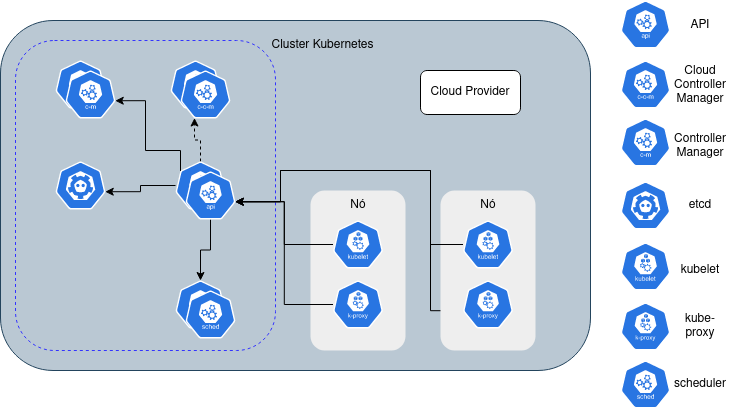
\includegraphics[scale=0.54]{images/kubernetes-components.png}
\caption{Componentes que compõe a arquitetura do Kubernetes e comunicações entre si.}
\label{fig:kubernetes:components}
\end{figure}

Como visto na figura, temos diversos componentes que juntos trabalham para
prover as funcionalidades do \textit{framework} do Kubernetes:

\begin{itemize}
    \item kube-apiserver: é a API do Kubernetes, onde estão definidos os tipos
    de recursos que o \textit{cluster} possui, realiza a interface de acesso aos
    dados que ficam armazenados em banco de dados. Permite a criação e administração
    dos recursos através desta API através de acesso de dados CRUD (\textit{Create},
    \textit{Retrieve}, \textit{Update}, \textit{Delete}).
    \item etcd: não é desenvolvido pelo Kubernetes, mas, é utilizado para armazenar
    todos os metadados do \textit{cluster}, como por exemplo, em que nó um
    contêiner está sendo executado e quais outros contêineres podem acessar via
    HTTP este contêiner. Neste banco de dados de chave/valor também são armazenados
    o estado desejável dos recursos que o Kubernetes está administrando.
    \item kube-scheduler: aplicação que cuida da atribuição de um nó para um contêiner.
    Para escolher o melhor nó se faz uso de diversas políticas, como a definição dos
    recursos necessários do contêiner, é necessário que o nó possua os recursos e
    que os recursos gerais sejam utilizados da melhor forma no \textit{cluster},
    ou também se o nó possui alguma peculiaridade em anotação, como, por exemplo,
    uma GPU, o que é chamado de \textit{node affinity}.
    \item kube-controler-manager: todos os recursos da API do Kubernetes possuem
    um \textit{controller}(controlador) que controla a criação e administração
    destes recursos. Nesta aplicação, estão definidos a maioria dos controladores
    padrões do Kubernetes. Quando necessitamos estender a API, geralmente escrevemos
    novos controladores que executam separadamente destes.
    \item cloud-controller-manager: aplicação específica para \textit{clusters}
    que estejam sendo executados em serviços de nuvem, permitindo que o serviço defina
    como serão feitos os roteamentos de dados de rede e outras particularidades de
    acesso de rede na nuvem, por exemplo, abertura de portas e exposição das mesmas,
    protocolos de redes, DNS, entre outros.
\end{itemize}

Nem todo nó precisa executar o \textit{control plane}, mas, todos os nós que
executam contêineres do usuário precisam contar com três aplicações, o kubelet,
o kube-proxy e a \textit{runtime} de contêiner, como visto na Figura
\ref{fig:kubernetes:components}. O kubelet é responsável por administrar os
contêineres da máquina e assegurar que o contêiner é executado conforme a
definição de um Pod. Desta forma, é possível saber quais contêineres não são mais
necessários através das definições do estado almejado por cada recurso. O
kube-proxy implementa regras de rede para o nó que permitem que os contêineres
que este executa sejam acessíveis aos outros nós do \textit{cluster}, através
de registros DNS internos ao \textit{cluster}. Por fim, a \textit{runtime} de
contêineres é a responsável por de fato executar os contêineres do nó. O kubelet
se comunica com a \textit{runtime} de contêineres para que seja possível realizar
a administração dos contêineres, realizando ações que seriam feitas manualmente
por um usuário fora de um orquestrador, como escalar um contêiner.

\subsubsection{Pod}

O Pod é o conceito fundamental do Kubernetes. Um Pod é a encapsulação de
diversos contêineres de uma aplicação com significado lógico para estarem
executando juntos. Dentro de um Pod, as ferramentas do Linux, como cgroups e
namespaces, isolam os contêineres executando no Pod em um contexto
compartilhado, permitindo a comunicação entre os contêineres e compartilhamento
de recursos. O Pod é definido, como todo recurso do Kubernetes, através de um
arquivo YAML ou JSON, contendo a imagem que será utilizada, os recursos e
também os contêineres que serão utilizados \cite{kubernetes:pod}. O próprio
Kubernetes executa algumas de suas aplicações internas em Pods, como o próprio
kube-apiserver. Toda aplicação que executa no Kubernetes executa através de um
Pod, que é o recurso mínimo para que possamos utilizar o Kubernetes.

\subsubsection{Deployment/StatefulSet}

Para administrar Pods no Kubernetes utilizamos o Deployment ou o StatefulSet.
A principal diferença entre os dois é que o último permite a utilização de
volumes persistentes para armazenar dados entre reinicializações dos Pods.
Eles permitem definir os estado que queremos que nosso Pods permaneçam, este
estado está relacionado principalmente ao número de réplicas deste Pod e
também da versão de imagem de contêiner que eles devem estar. O Deployment
ou StatefulSet lida com toda a parte de criar novos Pods e seus contêineres,
de reiniciá-los, pará-los ou atualizá-los através de um controlador do
kube-controller-manager \cite{kubernetes:deployment}. Estes recursos permitem
que o Kubernetes possa administrar as aplicações que ele executa através de
outros recursos, como o ReplicaSet, que é a definição da quantidade de réplicas
que deve ser mantida para cada um dos serviços.

\subsubsection{Volumes}

Para o armazenamento de dados persistentes, o Kubernetes utiliza o conceito
de Volumes, que é uma abstração sobre uma localização de dados
persistentes. Existem diferentes tipos de volumes que permitem que sejam
utilizadas implementações de diferentes provedores de serviços em nuvem ou
até mesmo de discos rígidos das máquinas em que se está executando o
\textit{cluster} do Kubernetes \cite{kubernetes:volumes}.

Os Volumes do Kubernetes funcionam de maneira diferente dos do
Docker, sendo que no último é mais desorganizado, onde, é apenas disponível para o
disco local ou outro contêiner. Os Volumes do Kubernetes permitem
que seja compartilhando um volume entre diversos Pods através de permissões
dos volumes que são solicitadas para os Pods como PersistentVolumeClaim para os
PersistentVolumes \cite{kubernetes:persistent-volumes}. Nas reinicializações
de Pods com PersistentVolumeClaims é assegurado que eles receberão acesso
ao mesmo volume novamente, persistindo os dados armazenados da aplicação.
Isto não permite o salvamento de dados em memória, que não são salvos em
persistência de dados, mas, no contexto da aplicação.

\subsubsection{Controllers}

Todos os recursos definidos no Kubernetes são controlados pelos chamados
\textit{Controllers}. Estes controladores ouvem a mudanças nos estados dos recursos
a partir de monitoramento da API do Kubernetes, kube-apiserver, e executam passos
para atingir os objetivos de estado que os recursos na API necessitam. O
Kubernetes provê alguns recursos padrões, como Pods, Jobs e Volumes e
todos estes possuem um controlador para controlar o estado desejado de
cada um dos recursos \cite{kubernetes:controllers}.

Também podemos adicionar recursos através de controladores personalizados,
estes são criados em qualquer linguagem de programação e também se comunicam
com o kube-apiserver. Com isso, é possível estender, por exemplo, a
funcionalidade do StatefulSet Controller, a partir de monitoramento dos
recursos que ele administra. Com isso, podemos, por exemplo, adicionar novas
funcionalidades para monitorar Pods e criar funcionalidades como servidores
de \textit{reverse proxy} \cite{kubernetes:controllers}.

\section{Serviços Stateful e Stateless}

De modo geral, quando executamos uma aplicação ou um serviço em produção,
temos dois tipos de possibilidade de aplicações. Temos as aplicações que
não necessitam saber do estado de execução da aplicação, como, por exemplo,
a instrução que estava sendo executada. Aplicações que precisam
apenas acessar um banco de dados e servir dados, como uma API HTTP, não
possuem necessidade de permanecer o estado da memória ou mesmo de saber a
instrução sendo executada em determinado momento. Chamamos este tipo de
aplicação/serviço de \textit{Stateless}, ou seja, sem estado. A maioria das
aplicações desenvolvidas para microsserviços são desenvolvidas através
deste padrão \cite{vayghan2021kubernetes}.

No caso de aplicações mais críticas, que necessitam de um estado de execução,
como, por exemplo, uma aplicação que se comunica com clientes e mantém estado
do acesso de cada cliente e suas execuções em memória. Estas aplicações/serviços
nós chamamos do tipo \textit{Stateful}, ou seja, com estado. Estas, em geral,
tem menos tolerância a falhas, por exemplo, se ela falhar perdemos todo o estado
da aplicação e não teremos a mesma aplicação executando quando ela reiniciar,
é interessante que possamos de alguma forma salvar este estado nos casos de falha
\cite{vayghan2021kubernetes}.

O estado da aplicação em geral consiste do estado do processo pai e filhos
executando na aplicação. Este estado contém, por exemplo, como as páginas
de memória estão em determinado momento. Desta forma, temos exatamente o
estado da execução, mas, não temos conhecimento de como ela nele. Não seria
interessante para a aplicação salvar estes valores em persistência, pois,
seria necessária muita instrumentação \cite{oh2018stateful}.

\subsection{etcd}

O \textit{etcd} consiste de um banco de dados de chave/valor distribuído.
A distribuição e replicação dos dados se dá por um algoritmo de eleição de
líderes, logo, ele é tolerante a falhas e consistente. \cite{etcd}

Por se tratar de um banco de dados distribuídos, ele é adequado para
utilização em \textit{clusters}, e, por isso, é utilizado por padrão no
Kubernetes para armazenar metadados dos seus recursos. Também é comum que
controladores customizados do Kubernetes utilizem este para armazenamento
de seus metadados \cite{kubernetes:etcd}.

\section{Checkpointing/Restore}

A técnica de\textit{Checkpoint/Restore} permite o salvamento do estado de
uma aplicação \textit{Stateful} e, posteriormente, a restauração da
aplicação a partir do ponto de salvamento passado. Em geral a técnica
consiste em obter uma cópia da execução em memória da aplicação, salvar o
contexto em uma imagem que poderá ser armazenada em armazenamento sólido e
persistente. Quando há a necessidade de se recuperar o estado da aplicação
a imagem que temos é utilizada para recuperar o estado para o momento em
que ocorreu o salvamento da imagem \cite{laadan2010linux}.

Esta técnica pode ser utilizada para tolerância a falhas no caso de aplicações
que quando falham necessitam do estado de recuperação \cite{muller2022architecture}
\cite{Chen2015/10}, aplicações \textit{Stateful}. Nesta técnia temos cópias
dos estados anteriores da aplicação e podemos recuperá-la mais rapidamente.
Outra possibilidade também é aumentar a disponibilidade dos serviços através
do salvamento do estado e posterior recuperação dele \cite{vayghan2021kubernetes}.
Embora, a técnica de \textit{Checkpoint/Restore} tenha o objetivo de salvar um
estado e depois recuperá-lo, ela pode ser utilizada para outras finalidades não
envolvidas exatamente nessa linha, como migração de aplicações entre nós de um
\textit{cluster} \cite{Chen2015/10}.

\subsection{CRIU}

CRIU é um projeto que implementa \textit{Checkpoint/Restore} no Linux no
userspace, o acrônimo da aplicação se dá justamente por isso,
\textit{Checkpoint/Restore in Userspace}. Ele trabalha com o conceito de
congelar a execução de um processo, salvar seu estado de execução no disco,
que depois pode ser utilizado para recuperar a aplicação exatamente no
momento em que ela parou. Como contêineres são isoluções em cima das
ferramentas do Linux, é possível realizar o salvamento de estado de
contêineres utilizando o CRIU \cite{criu}.

Algumas \textit{runtimes} de contêineres possuem o suporte de
\textit{Checkpoint/Restore} implementado com o auxílio do CRIU, é o caso
do containerd. Por usar runc para construção do \textit{backend} da
\textit{runtime}, que possui o CRIU integrado, comandos na
interface de linha de comando do containerd foram criados para realizar o
\textit{Checkpoint/Restore}. Desta forma, utilizando o Kubernetes com
containerd também é possível realizar \textit{Checkpoint/Restore} dos
contêineres, não de forma nativa, mas se aproveitando das funcionalidades
do containerd através do CRIU e a comunicação com as APIs tanto do containerd
quanto do Kubernetes.

\section{Event Sourcing}

O padrão de projeto \textit{Event Sourcing} cria eventos sobre ações em um
sistema e, armazena estes em fluxos ordenados \cite{event-sourcing},
através de um versionamento da ordem. Então, quando uma ação é feita no sistema
temos a emissão de um novo evento para um determinado fluxo. Estes são ordenados
pela versão em que são entregues. Uma vantagem deste modelo é a possibilidade
de alcançar o estado da aplicação em um determinado momento apenas reprojetando
os eventos, ou seja, ao emitir os mesmos eventos em ordem até um determinado
momento no tempo, e, por momento se entende a última versão desejada
\cite{event-sourcing}.

Este padrão permite uma grande forma de auditoria ao armazenar as ações
feitas pelo sistema e permite encontrar incosistências com grande facilidade
ao reprojetar eventos até o ponto de uma falha. Também é possível adicionar
um \textit{snapshotter} que captura o estado do sistema em determinado
momento, e, não será necessário reprojetar todos os eventos desde de o início
do sistema, economizando tempo de processamento \cite{event-sourcing}.
